% 注意事项:编译两次,以确保目录、页码完整显示

\def\allfiles{}

\documentclass[14pt,a4paper,UTF8,twoside]{article}

% Formatting Packages ——————————————————————————————————————
\usepackage{multicol}
\usepackage{multirow}
\usepackage{enumitem}
\usepackage{indentfirst}
\usepackage[toc]{multitoc}

% Math & Physics Packages ————————————————————————————
\usepackage{amsmath, amsthm, amsfonts, amssymb}
\usepackage{setspace}
\usepackage{physics}
\usepackage{cancel}
\usepackage{nicefrac}
\usepackage{unicode-math} % 允许数学公式使用特定字体
\usepackage{mdframed}

% Image-related Packages —————————————————————————————
\usepackage{float} % 浮动体环境
\usepackage{subcaption} % 子图包
\usepackage{pgfgantt}
\usepackage{graphics, graphicx}
\usepackage{tikz, tikz-qtree}
\usetikzlibrary{arrows.meta, positioning, shapes}
\usetikzlibrary{shapes.geometric}
\tikzstyle{node_style} = [rectangle, rounded corners, draw, align=center, text width=3cm, minimum height=0.65cm]
\tikzstyle{arrow_style} = [thick, ->, >=stealth]

\usepackage{pgfplots}
\pgfplotsset{compat=1.18}
\usepackage{xcolor}
\usepackage{fourier-orns}
\usepackage{lipsum}

% Colour Palette ——————————————————————————————————————
\definecolor{merah}{HTML}{F4564E}
\definecolor{merahtua}{HTML}{89313E}
\definecolor{biru}{HTML}{60BBE5}
\definecolor{birutua}{HTML}{412F66}
\definecolor{hijau}{HTML}{59CC78}
\definecolor{hijautua}{HTML}{366D5B}
\definecolor{kuning}{HTML}{FFD56B}
\definecolor{jingga}{HTML}{FBA15F}
\definecolor{ungu}{HTML}{8C5FBF}
\definecolor{lavender}{HTML}{CBA5E8}
\definecolor{merjamb}{HTML}{FFB6E0}
\definecolor{mygray}{HTML}{E6E6E6}
\definecolor{mygreen}{rgb}{0,0.6,0}
\definecolor{mymauve}{rgb}{0.58,0,0.82}

% Theorems ————————————————————————————————————————————
\usepackage{tcolorbox}
\usepackage{changepage}
\tcbuselibrary{skins,breakable,theorems}

\newcounter{hitung}
\setcounter{hitung}{\thesection}

\makeatletter
	% Proof 证明如下
	\def\tcb@theo@widetitle#1#2#3{\hbox to \textwidth{\textsc{\large#1}\normalsize\space#3\hfil(#2)}}
	\tcbset{
		theorem style/theorem wide name and number/.code={ \let\tcb@theo@title=\tcb@theo@widetitle},
		proofbox/.style={skin=enhancedmiddle,breakable,parbox=false,boxrule=0mm,
			check odd page, toggle left and right, colframe=black!20!white!92!hijau,
			leftrule=8pt, rightrule=0mm, boxsep=0mm,arc=0mm, outer arc=0mm,
			left=3mm,right=3mm,top=0mm,bottom=0mm, toptitle=0mm,
			bottomtitle=0mm,colback=gray!3!white!98!biru, before skip=8pt, after skip=8pt,
			before={\par\vskip-2pt},after={\par\smallbreak},
		},
	}
	\newtcolorbox{ProofBox}{proofbox}
	\makeatother
	
	\let\realproof\proof
	\let\realendproof\endproof
	\renewenvironment{proof}[1][Prove:]{\ProofBox\strut\textsc{#1}\space}{\endProofBox}
        \AtEndEnvironment{proof}{\null\hfill$\blacksquare$}
        % Definition 定义环境
	\newtcbtheorem[use counter=hitung, number within=section]{dfn}{定义}
	{theorem style=theorem wide name and number,breakable,enhanced,arc=3.5mm,outer arc=3.5mm,
		boxrule=0pt,toprule=1pt,leftrule=0pt,bottomrule=1pt, rightrule=0pt,left=0.2cm,right=0.2cm,
		titlerule=0.5em,toptitle=0.1cm,bottomtitle=-0.1cm,top=0.2cm,
		colframe=white!10!biru,
		colback=white!90!biru,
		coltitle=white,
		shadow={1.3mm}{-1.3mm}{0mm}{gray!50!white}, % 添加阴影
        coltext=birutua!60!gray, title style={white!10!biru}, before skip=8pt, after skip=8pt,
		fonttitle=\bfseries,fontupper=\normalsize}{dfn}

	% 答题卡
	\newtcbtheorem[use counter=hitung, number within=section]{ans}{解答}
	{theorem style=theorem wide name and number,breakable,enhanced,arc=3.5mm,outer arc=3.5mm,
		boxrule=0pt,toprule=1pt,leftrule=0pt,bottomrule=1pt, rightrule=0pt,left=0.2cm,right=0.2cm,
		titlerule=0.5em,toptitle=0.1cm,bottomtitle=-0.1cm,top=0.2cm,
		colframe=white!10!biru,
		colback=white!90!biru,
		coltitle=white,
		shadow={1.3mm}{-1.3mm}{0mm}{gray!50!white}, % 添加阴影
        coltext=birutua!60!gray, title style={white!10!biru}, before skip=8pt, after skip=8pt,
		fonttitle=\bfseries,fontupper=\normalsize}{ans}

	% Axiom
	\newtcbtheorem[use counter=hitung, number within=section]{axm}{公理}
	{theorem style=theorem wide name and number,breakable,enhanced,arc=3.5mm,outer arc=3.5mm,
		boxrule=0pt,toprule=1pt,leftrule=0pt,bottomrule=1pt, rightrule=0pt,left=0.2cm,right=0.2cm,
		titlerule=0.5em,toptitle=0.1cm,bottomtitle=-0.1cm,top=0.2cm,
		colframe=white!10!biru,colback=white!90!biru,coltitle=white,
		shadow={1.3mm}{-1.3mm}{0mm}{gray!50!white!90}, % 添加阴影
        coltext=birutua!60!gray,title style={white!10!biru},before skip=8pt, after skip=8pt,
		fonttitle=\bfseries,fontupper=\normalsize}{axm}
 
	% Theorem
	\newtcbtheorem[use counter=hitung, number within=section]{thm}{定理}
	{theorem style=theorem wide name and number,breakable,enhanced,arc=3.5mm,outer arc=3.5mm,
		boxrule=0pt,toprule=1pt,leftrule=0pt,bottomrule=1pt, rightrule=0pt,left=0.2cm,right=0.2cm,
		titlerule=0.5em,toptitle=0.1cm,bottomtitle=-0.1cm,top=0.2cm,
		colframe=white!10!merah,colback=white!75!pink,coltitle=white, coltext=merahtua!80!merah,
		shadow={1.3mm}{-1.3mm}{0mm}{gray!50!white!90}, % 添加阴影
		title style={white!10!merah}, before skip=8pt, after skip=8pt,
		fonttitle=\bfseries,fontupper=\normalsize}{thm}
	
	% Proposition
	\newtcbtheorem[use counter=hitung, number within=section]{prp}{命题}
	{theorem style=theorem wide name and number,breakable,enhanced,arc=3.5mm,outer arc=3.5mm,
		boxrule=0pt,toprule=1pt,leftrule=0pt,bottomrule=1pt, rightrule=0pt,left=0.2cm,right=0.2cm,
		titlerule=0.5em,toptitle=0.1cm,bottomtitle=-0.1cm,top=0.2cm,
		colframe=white!10!hijau,colback=white!90!hijau,coltitle=white, coltext=hijautua!80!brown,
		shadow={1.3mm}{-1.3mm}{0mm}{gray!50!white}, % 添加阴影
		title style={white!10!hijau}, before skip=8pt, after skip=8pt,
		fonttitle=\bfseries,fontupper=\normalsize}{prp}


	% Example
	\newtcolorbox[use counter=hitung, number within=section]{cth}[1][]{breakable,
		colframe=white!10!jingga, coltitle=white!90!jingga, colback=white!85!jingga, coltext=black!10!brown!50!jingga, colbacktitle=white!10!jingga, enhanced, fonttitle=\bfseries,fontupper=\normalsize, attach boxed title to top left={yshift=-2mm}, before skip=8pt, after skip=8pt,
		title=Contoh~\thetcbcounter \ \ #1}

	% Catatan/Note
	\newtcolorbox{ctt}[1][]{enhanced, 
		left=4.1mm, borderline west={8pt}{0pt}{white!10!kuning}, 
		before skip=6pt, after skip=6pt, 
		colback=white!85!kuning, colframe= white!85!kuning, coltitle=orange!60!kuning!25!brown, coltext=orange!60!kuning!25!brown,
		fonttitle=\bfseries,fontupper=\normalsize, before skip=8pt, after skip=8pt,
		title=\underline{Annotation}  #1}
	
	% Komentar/Remark
	\newtcolorbox{rmr}[1][]{
		,arc=0mm,outer arc=0mm,
		boxrule=0pt,toprule=1pt,leftrule=0pt,bottomrule=5pt, rightrule=0pt,left=0.2cm,right=0.2cm,
		titlerule=0.5em,toptitle=0.1cm,bottomtitle=-0.1cm,top=0.2cm,
		colframe=white!10!kuning,colback=white!85!kuning,coltitle=white, coltext=orange!60!kuning,
		fonttitle=\bfseries,fontupper=\normalsize, before skip=8pt, after skip=8pt,
		title=Remark  #1}

\usepackage{booktabs} % 表格库
\usepackage{titlesec} % 标题库
\usepackage{fancyhdr} % 页眉页脚库
\usepackage[sorting=none]{biblatex}
\usepackage{array}
\addbibresource{references.bib} % 指定你的.bib文件名称

\date{} % 留空,以让编译时去除日期

%———————————————注意事项—————————————————%

% 1、如果编译显示失败,但没有错误信息,就是 filename.pdf 正在被占用
% 2、在文件夹中的终端使用 Windows > xelatex filename.tex 也可编译

%—————————————华东师范大学———————————————%

% 论文制作时须加页眉,页眉从中文摘要开始至论文末
% 偶数页码内容为:华东师范大学硕士学位论文,奇数页码内容为学位论文题目

%————————定义 \section 的标题样式————————%

% 注意:\chapter 等命令,内部使用的是 \thispagestyle{plain} 的排版格式
% 若需要自己加上页眉,实际是在用 \thispagestyle{fancy} 的排版格式
% 加上下面这一段指令,就能够让 \section 也使用 fancy 的排版格式
% 本质就是让目录、第一页也能够显示页眉、页脚

\fancypagestyle{plain}{
  \pagestyle{fancy}
}

\title{华东师范大学软件学院课程作业} % 模板
\titleformat{\section}
    {\normalfont\bfseries\Large} % 字体大小、字体系列(\bfseries 为加粗)
    {\thesection}{1em}{}

% ———————————设置章节的中文格式———————————%
\renewcommand\thesection{\chinese{section} \hspace{0pt}}
\renewcommand\thesubsection{\arabic{subsection} \hspace{0pt}}
% \renewcommand\thesubsubsection{\alph{subsubsection} \hspace{0pt}} % 字母编号
% \hspace{0pt} 是为了确保在章节编号和章节题目之间不要有空格,使得排版更为美观
    
%—————————————页面基础设置———————————————%

\usepackage{geometry}
\geometry{left=10mm, right=10mm, top=20mm, bottom=20mm}

%————————————设置页眉、页脚——————————————%

\pagestyle{fancy} % 设置 plain style 的属性

% 设置页眉

\fancyhead[RE]{\leftmark} % Right Even 偶数页右侧显示章名 \leftmark 最高级别章名
\fancyhead[LO]{\rightmark} % Left Odd 奇数页左侧显示节名 \rightmark 第二级别节名
\fancyhead[C]{华东师范大学软件学院课程作业} % Center 居中显示
\fancyhead[LE,RO]{~\thepage~} % 在偶数页的左侧,奇数页的右侧显示页码
\renewcommand{\headrulewidth}{1.2pt} % 页眉与正文之间的水平线粗细

% 设置页脚:在每页的右下脚以斜体显示书名

\fancyfoot[RO,RE]{\it Lab Report By \LaTeX} % 使用意大利斜体显示
\renewcommand{\footrulewidth}{0.5pt} % 页脚水平线宽度

%——————设置页码:在底部居中显示页码———————%

\usepackage{lastpage} % 页码数库
\pagestyle{fancy}
\fancyfoot[C]{\kaishu 第 \thepage 页 \ 共 \pageref{LastPage} 页} % LastPage 需要二次编译以获取总页数

%——————————————代码块设置———————————————%

\usepackage{listings} % 代码块包
\lstset {
    backgroundcolor=\color{white},   % choose the background color; you must add \usepackage{color} or \usepackage{xcolor}
    basicstyle=\footnotesize,        % the size of the fonts that are used for the code
    breakatwhitespace=false,         % sets if automatic breaks should only happen at whitespace
    breaklines=true,                 % sets automatic line breaking
    captionpos=bl,                   % sets the caption-position to bottom
    commentstyle=\color{mygreen},    % comment style
    deletekeywords={...},            % if you want to delete keywords from the given language
    escapeinside={\%*}{*},           % if you want to add LaTeX within your code
    extendedchars=true,              % lets you use non-ASCII characters; for 8-bits encodings only, does not work with UTF-8
    frame=single,                    % adds a frame around the code
    keepspaces=true,                 % keeps spaces in text, useful for keeping indentation of code (possibly needs columns=flexible)
    keywordstyle=\color{blue},       % keyword style
    % language=Python,               % the language of the code
    morekeywords={*,...},            % if you want to add more keywords to the set
    numbers=left,                    % where to put the line-numbers; possible values are (none, left, right)
    numbersep=5pt,                   % how far the line-numbers are from the code
    numberstyle=\tiny\color{mygray}, % the style that is used for the line-numbers
    rulecolor=\color{black},         % if not set, the frame-color may be changed on line-breaks within not-black text (e.g. comments (green here))
    showspaces=false,                % show spaces everywhere adding particular underscores; it overrides 'showstringspaces'
    showstringspaces=false,          % underline spaces within strings only
    showtabs=false,                  % show tabs within strings adding particular underscores
    stepnumber=1,                    % the step between two line-numbers. If it's 1, each line will be numbered
    stringstyle=\color{orange},      % string literal style
    tabsize=2,                       % sets default tabsize to 2 spaces
    % title=Python Code              % show the filename of files included with \lstinputlisting; also try caption instead of title
}

% 注释掉的部分用于后续插入代码,参数可调整,格式如下:

% 1、直接插入
% \begin{lstlisting}[language = ? , title = { ? } ]
%       Your code here.
% \end{lstlisting}

% 2、文件插入
% \lstinputlisting[language = C , title = ?.c] {filename.c}

%———————————————字体设置————————————————%

\usepackage{fontspec} % 允许设置字体
\usepackage[utf8]{inputenc}
\usepackage{ctex}
\linespread{1.2}
% \setCJKmainfont{SimSun} % 设置正文罗马族的 CJK 字体

%———————————————超链接设置——————————————%

\usepackage[hidelinks]{hyperref}
\hypersetup{
    pdfstartview=FitH, % 设置PDF文档打开时的初始视图为页面宽度适应窗口宽度(即页面水平适应)
    CJKbookmarks=true, % 用对CJK(中文、日文、韩文)字符的书签支持,确保这些字符在书签中正确显示
    bookmarksnumbered=true, % 书签带有章节编号。这对有章节编号的文档很有用
    bookmarksopen=true, % 文档打开时,书签树是展开的,方便查看所有书签
    colorlinks, % 启用彩色链接。这样,链接在PDF中会显示为彩色,而不是默认的方框
    pdfborder=001, % 设置PDF文档中链接的边框样式。001 表示链接周围没有边框,仅在单击时显示一个矩形
    linkcolor=blue, % 设置文档内部链接(如目录中的章节链接)的颜色为蓝色
    anchorcolor=blue, % 设置锚点链接(即目标在同一文档内的链接)的颜色为蓝色
    citecolor=blue, % 设置引用(如文献引用)的颜色为蓝色
}

%——————————————导言区结束,进入正文部分———————————————%

\begin{document}

\maketitle

\begin{center} % \extracolsep{\fill} 拉伸到页面最大宽度前,保证居中显示

  \begin{tabular*}{\textwidth}{@{\extracolsep{\fill}} l  l  l }
    \hline
    课程名称: &  年级:2023级本科  &  姓名: \\
    作业主题: & 学号:1023510 & 作业日期:2024/01/01 \\
    指导老师: & 组号: \\
    \hline
  \end{tabular*}

\end{center}

\tableofcontents % 目录也需要二次编译

\section{代码块}

\begin{lstlisting} [language = Python]
  import pandas as pd
  import numpy as np
\end{lstlisting}

\section{文内引用}

\begin{mdframed}[backgroundcolor=gray!10, linewidth=0.5pt, roundcorner=5pt]
	\textit{This is a reference.}
\end{mdframed}

\section{公式模块}

\subsection{解答 Colorbox}

\begin{ans}{解答}{解答}
	\[
		\text{Deralive}^{2} = \text{Dera}^{2} + \text{live}^{2}. \tag{Deralive Equation}
	\]
\end{ans}

\subsection{定理 Colorbox}

\begin{thm}{Pythagorean Theorem}{Pythagorean Theorem}
	Deralive is a normal person.
\end{thm}

\subsection{定义 Colorbox}

\begin{dfn}{Deralive}{}
	Deralive is a person.
\end{dfn}

\subsection{命题 Colorbox}

\begin{prp}{Deralive is a normal person.}{}
	Deralive is a normal person.
\end{prp}

\subsection{例子 Colorbox}

\begin{cth}
	Deralive is a normal person.
\end{cth}

\subsection{公理 Colorbox}

\begin{axm}{Axiom 1}{Axiom 1}
	Deralive is a normal person.
\end{axm}

\subsection{注释 Colorbox}

\begin{ctt}
	This is a annotation.
\end{ctt}

\subsection{评论 Colorbox}

\begin{rmr}
	This is a remark.
\end{rmr}

\subsection{证明 Colorbox}

\begin{proof}
	Deralive is alive.

	\[
		\because \ Deralive \ is \ alive.
	\]
	
	\[
		\therefore \ Deralive \ is \ alive.
	\]

	Q.E.D.
\end{proof}

\section{超链接}

\begin{itemize}
	\item 百度:\href{www.baidu.com}{\underline{www.baidu.com}}
\end{itemize}

\section{TCP 三次握手图}

\begin{center}
	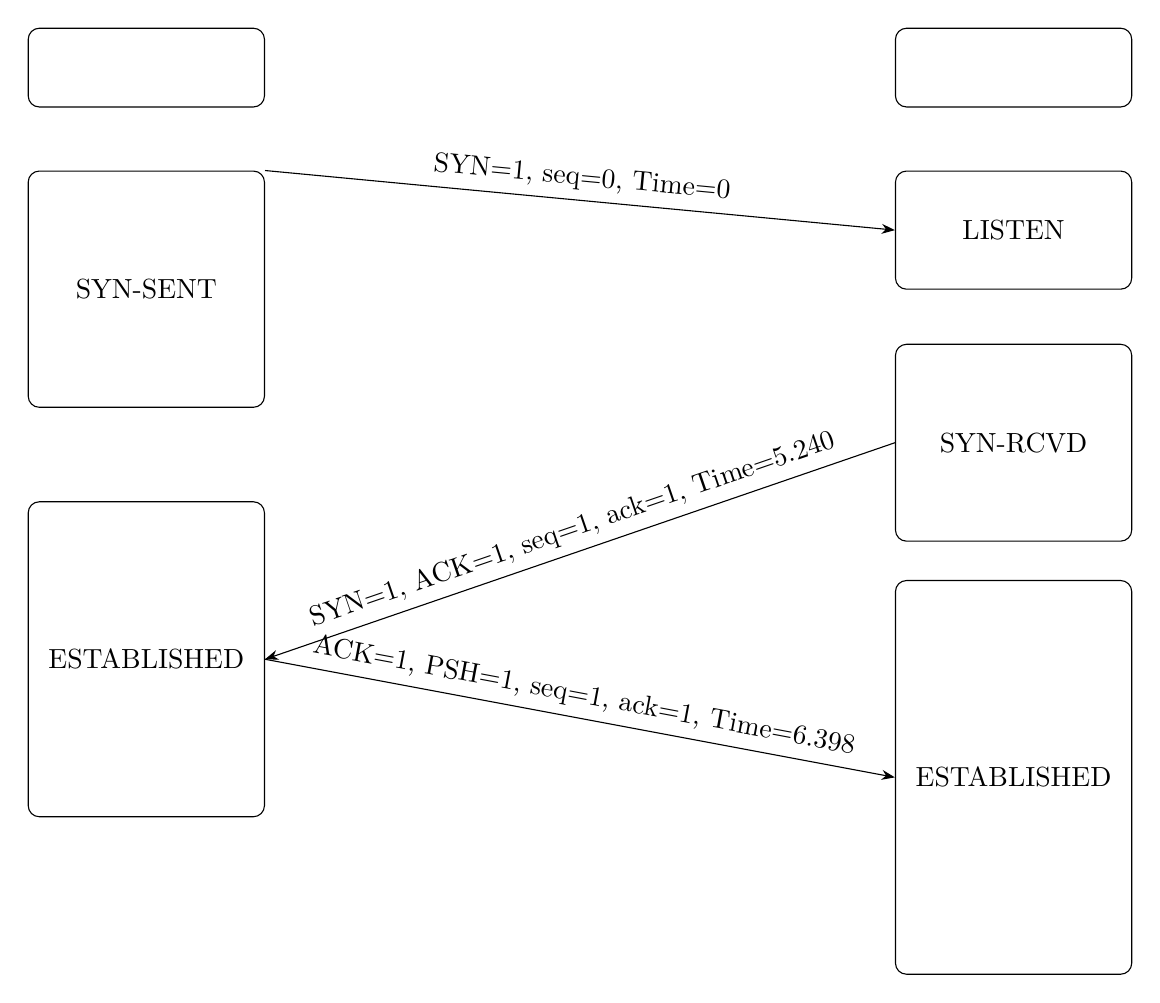
\begin{tikzpicture}[>=Stealth, node distance=2cm]
	
	% 客户机和服务器的节点
	\node[draw, rectangle, rounded corners, minimum height=1cm, minimum width=3cm] (client) {客户机};
	\node[draw, rectangle, rounded corners, minimum height=1cm, minimum width=3cm, right=8cm of client] (server) {服务器};
	
	% 状态节点
	\node[draw, rectangle, rounded corners, below=0.8cm of client, minimum height=3cm, minimum width=3cm] (syn_sent) {SYN-SENT};
	\node[draw, rectangle, rounded corners, below=0.8cm of server, minimum height=1.5cm, minimum width=3cm] (listen) {LISTEN};
	
	\node[draw, rectangle, rounded corners, below=5cm of client, minimum height=4cm, minimum width=3cm] (established_client) {ESTABLISHED};
	\node[draw, rectangle, rounded corners, below=3cm of server, minimum height=2.5cm, minimum width=3cm] (syn_rcvd) {SYN-RCVD};
	
	\node[draw, rectangle, rounded corners, below=6cm of server, minimum height=5cm, minimum width=3cm] (established_server) {ESTABLISHED};
	
	% 箭头和标签(通信过程)
	% 客户端发 SYN
	\draw[->] (syn_sent.north east) -- node[above, sloped] {SYN=1, seq=0, Time=0} (listen.west);
	
	% 服务器回应 SYN-ACK
	% \draw[->] (listen.west) -- node[above, sloped] {SYN=1, ACK=1, seq=0, ack=1, Time=5.240} (syn_rcvd.east);
	
	% 客户端发 ACK
	\draw[->] (syn_rcvd.west) -- node[above, sloped] {SYN=1, ACK=1, seq=1, ack=1, Time=5.240} (established_client.east);
	
	% 最终确认阶段
	\draw[->] (established_client.east) -- node[above, sloped] {ACK=1, PSH=1, seq=1, ack=1, Time=6.398} (established_server.west);
	
	\end{tikzpicture}
\end{center}

\section*{TikZ 节点的锚点参数}

在 TikZ 中,节点的锚点(anchor)定义了节点的不同参考位置,类似于方向上的“东南西北”。这些锚点允许你灵活地连接节点或对齐它们。

\begin{multicols}{3}
\subsection*{基础方向:东南西北}
\begin{itemize}
    \item \textbf{north}:顶部中心
    \item \textbf{south}:底部中心
    \item \textbf{east}:右侧中心
    \item \textbf{west}:左侧中心
\end{itemize}

\subsection*{组合方向:东北、西北等}
\begin{itemize}
    \item \textbf{north east}:右上角
    \item \textbf{north west}:左上角
    \item \textbf{south east}:右下角
    \item \textbf{south west}:左下角
\end{itemize}

\columnbreak

\subsection*{中心锚点}
\begin{itemize}
    \item \textbf{center}:节点的中心点
\end{itemize}

\subsection*{边缘锚点(中间位置)}
\begin{itemize}
    \item \textbf{mid}:整个节点的中间
    \item \textbf{mid north}:顶部中间
    \item \textbf{mid south}:底部中间
    \item \textbf{mid east}:右侧中间
    \item \textbf{mid west}:左侧中间
\end{itemize}

\subsection*{文字锚点(与文字对齐相关)}
\begin{itemize}
    \item \textbf{base}:与基线对齐
    \item \textbf{text}:与文本的边界对齐
    \item \textbf{text north},\textbf{text south} 等:文本边缘的方向
\end{itemize}

\end{multicols}

\newpage{}

\section{UDP 协议头的格式}

\begin{center}
	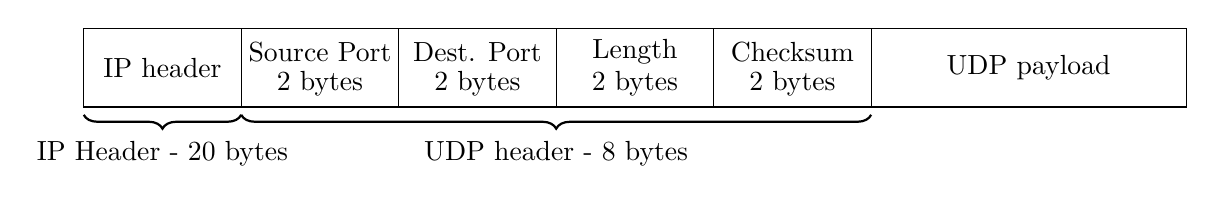
\begin{tikzpicture}[scale=1, transform shape]
	
	% 整个框架边界
	\draw (0, 0) rectangle (10, 1);
	
	% 划分 IP Header
	\draw (0, 0) -- (2, 0) -- (2, 1);
	\node at (1, 0.5) {IP header};
	
	% Source Port
	\draw (2, 0) -- (4, 0) -- (4, 1);
	\node at (3, 0.7) {Source Port};
	\node at (3, 0.3) {2 bytes};
	
	% Destination Port
	\draw (4, 0) -- (6, 0) -- (6, 1);
	\node at (5, 0.7) {Dest. Port};
	\node at (5, 0.3) {2 bytes};
	
	% Length
	\draw (6, 0) -- (8, 0) -- (8, 1);
	\node at (7, 0.7) {Length};
	\node at (7, 0.3) {2 bytes};
	
	% Checksum
	\draw (8, 0) -- (10, 0) -- (10, 1);
	\node at (9, 0.7) {Checksum};
	\node at (9, 0.3) {2 bytes};
	
	% UDP payload
	\draw (10, 0) rectangle (14, 1);
	\node at (12, 0.5) {UDP payload};
	
	% UDP header description with brace
	\draw [decorate, decoration={brace, amplitude=5pt, mirror}, thick] (2, -0.1) -- (10, -0.1);
	\node at (6, -0.6) {UDP header - 8 bytes};
	
	\draw [decorate, decoration={brace, amplitude=5pt, mirror}, thick] (0, -0.1) -- (2, -0.1);
	\node at (1, -0.6) {IP Header - 20 bytes};
	
	\end{tikzpicture}
\end{center}

\section{多行路线走势图}

\begin{center}
	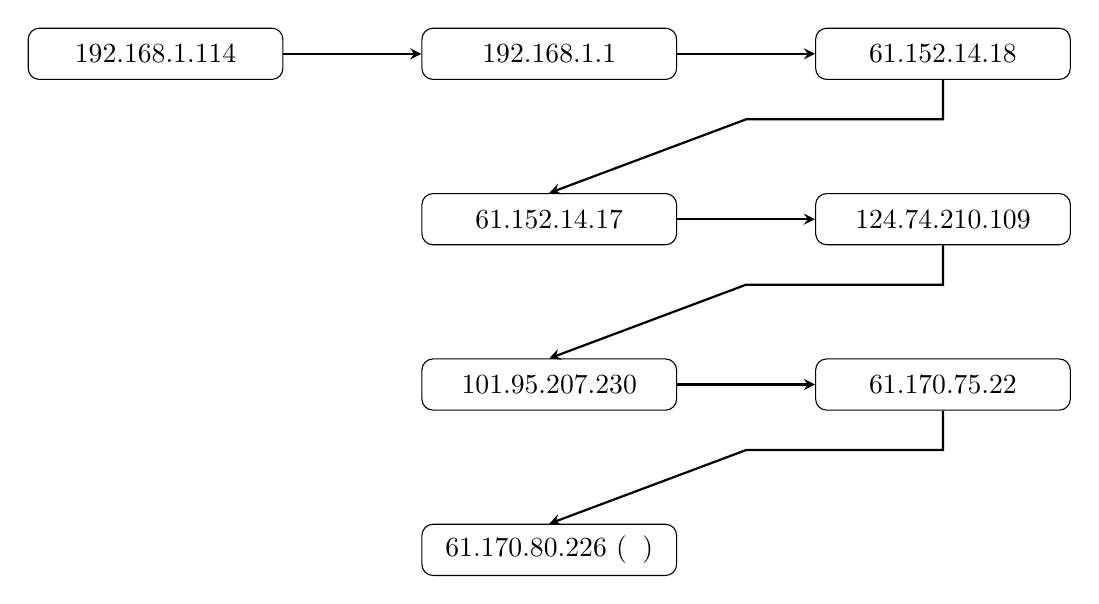
\begin{tikzpicture}[node distance=2cm and 3cm]
	
	  % 第一行
	  \node[node_style] (node0) {192.168.1.114}; % 新增节点
	  \node[node_style, right of=node0, xshift=3cm] (node1) {192.168.1.1};
	  \node[node_style, right of=node1, xshift=3cm] (node2) {61.152.14.18};
	  \draw[arrow_style] (node0.east) -- (node1.west); % 新增连接
	  \draw[arrow_style] (node1.east) -- (node2.west);
	  
	  % 第二行
	  \node[node_style, below of=node1, yshift=-0.1cm] (node3) {61.152.14.17};
	  \node[node_style, right of=node3, xshift=3cm] (node4) {124.74.210.109};
	  \draw[arrow_style] (node2.south) -- ++(0,-0.5) -- ++(-2.5,0) -- (node3.north);
	  \draw[arrow_style] (node3.east) -- (node4.west);
	  
	  % 第三行
	  \node[node_style, below of=node3, yshift=-0.1cm] (node5) {101.95.207.230};
	  \node[node_style, right of=node5, xshift=3cm] (node6) {61.170.75.22};
	  \draw[arrow_style] (node4.south) -- ++(0,-0.5) -- ++(-2.5,0) -- (node5.north);
	  \draw[arrow_style] (node5.east) -- (node6.west);
	  
	  % 第四行
	  \node[node_style, below of=node5, yshift=-0.1cm] (node7) {61.170.80.226 (目标)};
	  \draw[arrow_style] (node6.south) -- ++(0,-0.5) -- ++(-2.5,0) -- (node7.north);
	  
	  \end{tikzpicture}
\end{center}

\section{图表}

\subsection{三线图}

\[
\begin{array}{cccccc}
\toprule
F & SF & R & SV & M & T \\
\midrule
6.8 & 8.2 & 7.8 & 6.8 & 7.9 & \\
8.8 & 8.9 & 9.2 & 9.0 & 9.3 & \\
5.6 & 5.9 & 6.0 & 9.0 & 5.3 & \\
4.6 & 7.8 & 3.8 & 5.1 & 4.5 & \\
\bottomrule
\end{array}
\]

\subsection{多行居中表格}

\begin{table}[H]
	\centering
	\caption{作业三的数据}
	\begin{tabular}{|c|c|c|c|c|c|c|c|c|}
	  \hline
	  编号 & $x_1$ & $x_2$ & $x_3$ & $x_4$ & $x_5$ & $\rho_y$ & $y_1$ & $y_2$ \\
	  \hline
	  \multirow{2}{*}{1} & 8.6 & 9.1 & 9.2 & 8.8 & 8.9 & 0.01 & \multirow{2}{*}{8.927694} & 8.927671 \\
						 & 8.6 & 9.1 & 9.2 & 8.8 & 8.9 & 0.55 &                       & 9.114381 \\
	  \hline
	  \multirow{2}{*}{2} & 6.8 & 7.9 & 5.9 & 6.6 & 6.1 & 0.01 & \multirow{2}{*}{6.614913} & 6.614570 \\
						 & 6.8 & 7.9 & 5.9 & 6.6 & 6.1 & 0.55 &                       & 6.596355 \\
	  \hline
	  \multirow{2}{*}{3} & 9.1 & 9.9 & 8.9 & 8.8 & 7.8 & 0.01 & \multirow{2}{*}{8.859329} & 8.859071 \\
						 & 9.1 & 9.9 & 8.9 & 8.8 & 7.8 & 0.55 &                       & 8.845068 \\
	  \hline
	  \multirow{2}{*}{4} & 3.5 & 4.2 & 5.6 & 4.9 & 5.2 & 0.01 & \multirow{2}{*}{4.695127} & 4.694559 \\
						 & 3.5 & 4.2 & 5.6 & 4.9 & 5.2 & 0.55 &                       & 4.663374 \\
	  \hline
	\end{tabular}
\end{table}

\subsection{更美观的表格}

\begin{table}[H]
	\centering
	\begin{tabular}{c|ccccccccc|c|c}
	\toprule
	\textbf{Index} &\textbf{1} & \textbf{2} & \textbf{3} & \textbf{4} & \textbf{5} & \textbf{6} & \textbf{7} & \textbf{8} & \textbf{9} & \textbf{Value} & \textbf{Level} \\
	\midrule
	10 & 7.6628 & 5.4788 & 6.3639 & 7.0000 & 7.8744 & 3.7417 & 10.0000 & 9.0000 & 4.5721  & 6.4071 & II \\
	11 & 8.3255 & 3.2854 & 7.6053 & 7.6053 & 9.6583 & 8.3666 & 10.0000 & 9.0000 & 10.0000 & 7.2713 & II \\
	12 & 8.3255 & 3.2854 & 8.3666 & 9.0000 & 9.6583 & 8.3666 & 10.0000 & 9.0000 & 10.0000 & 7.6010 & II \\
	13 & 8.3255 & 3.2854 & 7.6053 & 7.6053 & 9.6583 & 8.3666 & 10.0000 & 9.0000 & 10.0000 & 7.2713 & II \\
	14 & 8.3255 & 3.2854 & 7.6053 & 7.6053 & 9.6583 & 8.3666 & 10.0000 & 9.0000 & 10.0000 & 7.2713 & II \\
	15 & 8.3255 & 3.2854 & 8.0722 & 9.0000 & 9.6583 & 8.3666 & 10.0000 & 9.0000 & 10.0000 & 7.5467 & II \\
	16 & 8.3255 & 3.2854 & 7.6053 & 7.6053 & 9.6583 & 8.3666 & 10.0000 & 9.0000 & 10.0000 & 7.2713 & II \\
	17 & 8.3255 & 3.2854 & 7.6053 & 7.6053 & 9.6583 & 8.3666 & 10.0000 & 9.0000 & 9.6481  & 7.2479 & II \\
	\bottomrule
	\end{tabular}
	\caption{结果表}
\end{table}

\subsection{矩阵}

\[
\mathbf{A} = 
\begin{bmatrix}
    1 & 1/2 & 3 & 2 & 1/2 \\
    2 & 1 & 2 & 3 & 2 \\
    1/3 & 1/2 & 1 & 2 & 1/3 \\
    1/2 & 1/3 & 1/2 & 1 & 2 \\
    2 & 1/2 & 3 & 1/2 & 1 \\
\end{bmatrix}
\]

\subsection{多格表格}

\begin{table}[H]
	\centering
	\renewcommand{\arraystretch}{1.5} % 设置行高
	\begin{tabular}{|c|c|c|c|c|c|c|c|c|}
	\hline
	\textbf{进程} & \multicolumn{4}{|c|}{\textbf{Allocation}} & \multicolumn{4}{|c|}{\textbf{Max}} \\ \hline
	 & A & B & C & D & A & B & C & D \\ \hline
	$P_0$ & 3 & 0 & 1 & 4 & 5 & 1 & 1 & 7 \\ \hline
	$P_1$ & 2 & 2 & 1 & 0 & 3 & 2 & 1 & 1 \\ \hline
	$P_2$ & 3 & 1 & 2 & 1 & 3 & 3 & 2 & 1 \\ \hline
	$P_3$ & 0 & 5 & 1 & 0 & 4 & 6 & 1 & 2 \\ \hline
	$P_4$ & 4 & 2 & 1 & 2 & 6 & 3 & 2 & 5 \\ \hline
	\end{tabular}
	\caption{系统资源快照}
\end{table}

\section{建模图}

\begin{multicols}{2} % 分为两栏

    % 左侧流程图
    \noindent\textbf{流程图:}
    \begin{center}
        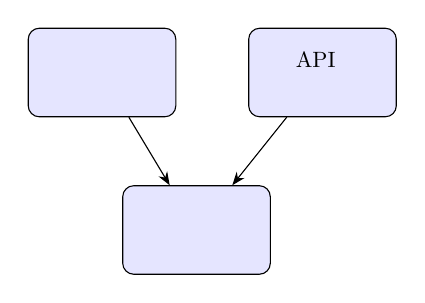
\begin{tikzpicture}[node distance=1cm, scale=0.8, transform shape]
            \tikzstyle{block} = [rectangle, draw, fill=blue!10, text width=6em, text centered, rounded corners, minimum height=4em]
            \tikzstyle{line} = [draw, -{Stealth}]
        
            % 定义节点
            \node[block] (start) {依赖库调 \\ 用分析};
            \node[block, right of=start, xshift=2.5cm] (api) {API 差 \\ 异分析};
            \node[block, below of=start, xshift=1.5cm, yshift=-1.5cm] (compatibility) {软件间兼容 \\ 性分析};
        
            % 添加箭头
            \path [line] (start) -- (compatibility);
            \path [line] (api) -- (compatibility);
        \end{tikzpicture}
    \end{center}
    
    \columnbreak % 分栏分隔符

    % 右侧简要分析信息
    \textbf{流程分析:}  

    主软件通过调用依赖库的 API,检测当前版本与默认版本之间的差异,评估这些差异是否引发兼容性问题。  

    \vspace{0.5cm}

    当直接依赖软件的某个抽象类中添加了新的抽象方法时,只有主软件继承了该类才会出现兼容性问题。
    
\end{multicols}

\begin{multicols}{2} % 分为两栏

    \begin{center}
        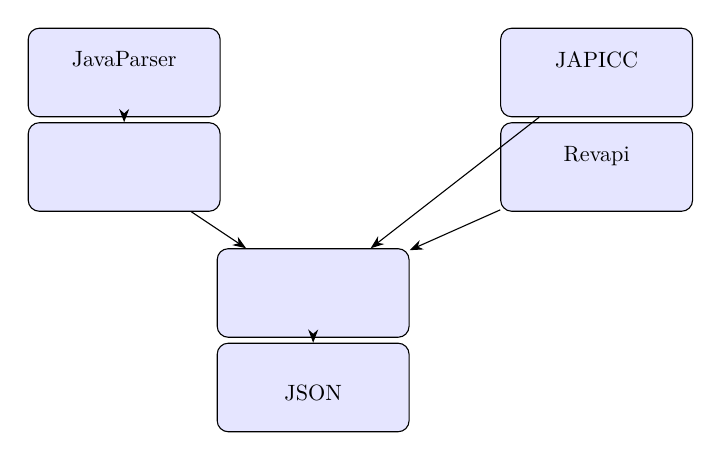
\begin{tikzpicture}[node distance=1.5cm, scale=0.8, transform shape]
            \tikzstyle{block} = [rectangle, draw, fill=blue!10, text width=8em, text centered, rounded corners, minimum height=4em]
            \tikzstyle{line} = [draw, -{Stealth}]
        
            % 定义节点
            \node[block] (parser) {JavaParser \\ 解析源代码};
            \node[block, below of=parser] (extract) {提取与依赖库相关的调用};
            \node[block, right of=parser, xshift=6cm] (japicc) {JAPICC \\ 差异检测};
            \node[block, below of=japicc] (revapi) {Revapi \\ 差异检测};
    
            % 中间节点 - 移动到中心
            \node[block, below of=extract, xshift=3cm, yshift=-0.5cm] (compat) {根据规则进行 \\ 兼容性分析};
            \node[block, below of=compat] (output) {兼容性度量 \\ 输出JSON报告};
    
            % 添加箭头
            \path [line] (parser) -- (extract);
            \path [line] (japicc) -- (compat);
            \path [line] (revapi) -- (compat);
            \path [line] (extract) -- (compat);
            \path [line] (compat) -- (output);
        \end{tikzpicture}
    \end{center}
    
    \columnbreak % 分栏分隔符

    % 右侧简要分析信息
    \noindent\textbf{流程分析:}  
    \begin{itemize}
        \item JavaParser 解析主软件源码,提取对依赖库的调用。  
        \item 通过工具检测新旧版本依赖库之间的 API 差异。  
        \item 基于兼容性规则分析差异的影响,度量兼容性问题,并输出 JSON 格式的结果报告。  
    \end{itemize}

    \noindent\textbf{注意事项:}
    当一个API调用受到多个API差异的影响时,受到影响的严重程度取高值。
    \[
    \textbf{High > Medium > Low > No}
    \]

\end{multicols}

\section{甘特图}

\begin{figure}[H]
    \begin{center}
    
    \begin{ganttchart}[y unit title=0.4cm,
    y unit chart=0.5cm,
    vgrid,hgrid, 
    title label anchor/.style={below=-1.6ex},
    title left shift=.05,
    title right shift=-.05,
    title height=1,
    progress label text={},
    bar height=0.7,
    group right shift=0,
    group top shift=.6,
    group height=.3]{1}{20}
    %labels
    \gantttitle{Cycle}{20} \\
    %tasks
    \ganttbar{FCFS}{1}{2}
    \ganttbar{FCFS}{3}{3}
    \ganttbar{FCFS}{4}{11}
    \ganttbar{FCFS}{12}{15}
    \ganttbar{FCFS}{16}{20} \\ 
    \ganttbar{SJF}{1}{1}
    \ganttbar{SJF}{2}{3}
    \ganttbar{SJF}{4}{7}
    \ganttbar{SJF}{8}{12}
    \ganttbar{SJF}{13}{20} \\
    \ganttbar{Priority}{1}{8}
    \ganttbar{Priority}{9}{13}
    \ganttbar{Priority}{14}{15}
    \ganttbar{Priority}{16}{19} 
    \ganttbar{Priority}{20}{20} \\
    \ganttbar{RR}{1}{2}
    \ganttbar{RR}{3}{3}
    \ganttbar{RR}{4}{5}
    \ganttbar{RR}{6}{7}
    \ganttbar{RR}{8}{9}
    \ganttbar{RR}{10}{11}
    \ganttbar{RR}{12}{13}
    \ganttbar{RR}{14}{15}
    \ganttbar{RR}{16}{17}
    \ganttbar{RR}{18}{18}
    \ganttbar{RR}{19}{20} \\
    \end{ganttchart}
    \end{center}
    \caption{Gantt Chart}

\end{figure}

\end{document}